\documentclass[12pt, titlepage, french]{report}
% Extra note : this preamble creates document that are meant to be used inside the multicols environment. See the documentation on internet for further information.

%% -----------------------------
%% Encoding packages
%% -----------------------------
\usepackage[utf8]{inputenc}
\usepackage[T1]{fontenc}
\usepackage{babel}
\usepackage{lmodern}
%
%%% -----------------------------
%%% Variable definition
%%% -----------------------------
%\def\auteur{Alec James van Rassel}
%\def\BackgroundColor{white}
%
%%% -----------------------------
%%% Margin and layout
%%% -----------------------------
%% Determine the margin for cheatsheet
\usepackage[hmargin=1cm, vmargin=1.7cm]{geometry}
\usepackage{multicol}

%% -----------------------------
%% URL and links
%% -----------------------------
\usepackage{hyperref}
\hypersetup{colorlinks = true, urlcolor = white, linkcolor = black}

%% -----------------------------
%% Document policy (uncomment only one)
%% -----------------------------
%	\usepackage{concrete}
%	\usepackage{mathpazo}
%	\usepackage{frcursive} %% permet d'écrire en lettres attachées
%	\usepackage{aeguill}
%	\usepackage{mathptmx}
%	\usepackage{fourier} 

%% -----------------------------
%% Math configuration
%% -----------------------------
\usepackage[fleqn]{amsmath}
\usepackage{amsthm,amssymb,latexsym,amsfonts}
\usepackage{empheq}
\usepackage{numprint}
\usepackage{dsfont} % Pour avoir le symbole du domaine Z

% Mathematics shortcuts

\newcommand{\reels}{\mathbb{R}}
\newcommand{\entiers}{\mathbb{Z}}
\newcommand{\naturels}{\mathbb{N}}
\newcommand{\eval}{\biggr \rvert}
\usepackage{cancel}
\newcommand{\derivee}[1]{\frac{\partial}{\partial #1}}
\newcommand{\prob}[1]{\Pr \left( #1 \right)}
\newcommand{\esp}[1]{\mathrm{E} \left[ #1 \right]} % espérance
\newcommand{\variance}[1]{\mathrm{Var} \left( #1   \right)}
\newcommand{\covar}[1]{\mathrm{Cov} \left( #1   \right)}
\newcommand{\laplace}{\mathcal{L}}
\newcommand{\deriv}[2][]{\frac{\partial^{#1}}{\partial #2^{#1}}}
\newcommand{\e}[1]{\mathrm{e}^{#1}}
\newcommand{\te}[1]{\text{exp}\left\{#1\right\}}
\DeclareMathSymbol{\shortminus}{\mathbin}{AMSa}{"39}

% To indicate equation number on a specific line in align environment
\newcommand\numberthis{\addtocounter{equation}{1}\tag{\theequation}}

%
% Actuarial notation packages
%
\usepackage{actuarialsymbol}
\usepackage{actuarialangle}

%
% Matrix notation for math symbols (\bm{•})
%
\usepackage{bm}
% Matrix notation variable (bold style)
\newcommand{\matr}[1]{\mathbf{#1}}


%% -----------------------------
%% tcolorbox configuration
%% -----------------------------
\usepackage[most]{tcolorbox}
\tcbuselibrary{xparse}
\tcbuselibrary{breakable}
%%	-----------------------------
%%
%%	Arguments
%%	+	breakable: allows box to be split over several pages
%%	+	segmentation style: To customize the \tcbline seperator
%%	
%%	-----------------------------
%%
%%
%% Coloured box "definition" for definitions
%%
%%
%% Coloured box "definition2" for definitions
%%
\DeclareTColorBox{definitionNOHFILL}{ o }				% #1 parameter
{
	colframe=blue!60!green,colback=blue!5!white, % color of the box
	pad at break* = 0mm, 						% to split the box
	title = {#1},
	before title = {\faBook \quad },
	breakable
}
%%
%% Coloured box "definition2" for definitions
%%
\DeclareTColorBox{definitionNOHFILLsub}{ o }				% #1 parameter
{
	colframe=blue!40!green,colback=blue!5!white, % color of the box
	pad at break* = 0mm, 						% to split the box
	title = {#1},
	before title = {\faNavicon \quad }, %faBars  faGetPocket
	breakable
}
\DeclareTColorBox{theorems}{ o}			% #1 parameter
{
	enhanced,
	title = #1,
	colback=bluebell, % color of the box
	colframe=blue(pigment),
	colbacktitle=blue!80!black,
	fonttitle = \bfseries,
	boxed title style={size=small,colframe=purple!50!black} ,
	attach boxed title to top center = {yshift=-3mm,yshifttext=-1mm},
	left=0pt,
  	right=0pt,
    box align=center,
    ams align*
%  	top=-10pt
}
\DeclareTColorBox{distributions}{ o }			% #1 parameter
{
	enhanced,
	title = #1,
	colback=ashgrey, % color of the box
%	colframe=blue(pigment),
%	colframe=lightgray,	
	colbacktitle=aurometalsaurus,
	fonttitle = \bfseries,
	boxed title style={size=small,colframe=arsenic} ,
	attach boxed title to top center = {yshift=-3mm,yshifttext=-1mm},
%	left=0pt,
%  	right=0pt,
%    box align=center,
%    ams align*
%  	top=-10pt
}
\DeclareTColorBox{astuces}{ o }			% #1 parameter
{
	enhanced,
	title = #1,
	colback=beaublue, % color of the box
%	colframe=blue(pigment),
	colframe=ballblue,	
	colbacktitle=aurometalsaurus,
	fonttitle = \bfseries,
	boxed title style={size=small,colframe=arsenic} ,
	attach boxed title to top center = {yshift=-3mm,yshifttext=-1mm},
%	left=0pt,
%  	right=0pt,
%    box align=center,
%    ams align*
%  	top=-10pt
}
\DeclareTColorBox{outcomes}{ o }			% #1 parameter
{
	enhanced,
	title = #1,
	colback=bluebell, % color of the box
%	colframe=blue(pigment),
%	colframe=asparagus,	
	colbacktitle=airforceblue,
	fonttitle = \bfseries,
	boxed title style={size=small,colframe=arsenic} ,
	attach boxed title to top center = {yshift=-3mm,yshifttext=-1mm},
%	left=0pt,
%  	right=0pt,
%    box align=center,
%    ams align*
%  	top=-10pt
}
\DeclareTColorBox{ASM_chapter}{ o }			% #1 parameter
{
	enhanced,
	title = #1,
	colback=darkseagreen, % color of the box
%	colframe=blue(pigment),
%	colframe=asparagus,	
	colbacktitle=britishracinggreen,
	fonttitle = \bfseries,
	boxed title style={size=small,colframe=arsenic} ,
	attach boxed title to top center = {yshift=-3mm,yshifttext=-1mm},
	segmentation style = {dashed, white},
	breakable
%	left=0pt,
%  	right=0pt,
%    box align=center,
%    ams align*
%  	top=-10pt
}
\DeclareTColorBox{YTB_vids}{ o }			% #1 parameter
{
	enhanced,
	title = #1,
	colback=red_rectangle, % color of the box
%	colframe=blue(pigment),
%	colframe=asparagus,	
	colbacktitle=lava,
	fonttitle = \bfseries,
	boxed title style={size=small,colframe=arsenic} ,
	attach boxed title to top center = {yshift=-3mm,yshifttext=-1mm},
	segmentation style = {dashed, white},
	breakable
%	left=0pt,
%  	right=0pt,
%    box align=center,
%    ams align*
%  	top=-10pt
}
%%
%% Coloured box "algo" for algorithms
%%
\newtcolorbox{algo}[ 1 ]
{
	colback = blue!5!white,
	colframe = blue!75!black,
	fonttitle = \bfseries,title=#1
}
%%
%% Coloured box "formula" for formulas
%%
\newtcolorbox{formula}[ 1 ]
{
	colback = beaublue,
	colframe = airforceblue,
	fonttitle = \bfseries,title=#1
}
%%
%% Coloured box "CHPT_SUMM" pour résumés des chapitres de l'ASM
%%
\newtcolorbox{CHPT_SUMM}[ 1 ]
{
	colback = green!5!white,
	colframe = darkseagreen,
	breakable,
	fonttitle = \bfseries,title=#1
}
%%
%% Coloured box "FORMULA_SUMM" pour résumés des formules de l'ASM
%%
\newtcolorbox{FORMULA_SUMM}[ 1 ]
{
	colback = babyblueeyes,
	colframe = airforceblue,
	breakable,
	fonttitle = \bfseries,title=#1
}
%%
%% Coloured box "YTB_SUMM" pour résumés des vidéos Youtube
%%
\newtcolorbox{YTB_SUMM}[ 1 ]
{
	colback = red!5!white,
	colframe = darkterracotta,
	breakable,
%	    frame hidden,
	fonttitle = \bfseries,title=#1
}
\newtcolorbox[auto counter, list inside = CHPT]{YTB_SUMM_AUTO_NUMB}[ 2 ][]
{
	colback = red!5!white,
	colframe = darkterracotta,
	breakable,
	enhanced,
	fonttitle = \bfseries,
	title = Video~\thetcbcounter: #2, 		
%	title = #2,
	nameref = #2,
	after upper = {\addcontentsline{toc}{subsubsection}{\thetcbcounter: #2}},
%	phantomlabel = {#2},
	#1
}
%%
%% Coloured box "rappel" pour rappel de formules
%%
\DeclareTColorBox{rappel_enhanced}{ o }
{
	enhanced,
	title = #1,
	colback=lightgray, % color of the box
%	colframe=blue(pigment),
%	colframe=arsenic,	
	colbacktitle=arsenic,
	fonttitle = \bfseries,
	breakable,
	boxed title style={size=small,colframe=arsenic} ,
	attach boxed title to top center = {yshift=-3mm,yshifttext=-1mm},
}
%%
%% Coloured box "FORMULA_SUMM" pour résumés des formules de l'ASM
%%
%% -----------------------------
%% Graphics and pictures
%% -----------------------------
\usepackage{graphicx}
\usepackage{pict2e}
\usepackage{tikz}
%%
%%	Creates circle 
%%	Arguments:
%%	+	size
%%	+	colour
%%	
%%	Example:
%%	+	\tikzcircle[green, fill=blue]{1.5pt}
%%	+	\tikzcircle{2pt}
%%
\newcommand{\tikzcircle}[2][red,fill=red]{\tikz[baseline=-0.5ex]\draw[#1,radius=#2] (0,0) circle ;}


%% -----------------------------
%% insert pdf pages into document
%% -----------------------------
\usepackage{pdfpages}

%% -----------------------------
%% Color configuration
%% -----------------------------
\usepackage{color, soulutf8, colortbl}

%
%	Colour definitions
%
\definecolor{ceruleanblue}{rgb}{0.16, 0.32, 0.75}
\definecolor{darkterracotta}{rgb}{0.8, 0.31, 0.36}   % red pastel ish
\definecolor{lava}{rgb}{0.81, 0.06, 0.13}
\definecolor{wildwatermelon}{rgb}{0.99, 0.42, 0.52}  % red ish
\definecolor{bostonuniversityred}{rgb}{0.8, 0.0, 0.0} % rich red
\definecolor{asparagus}{rgb}{0.53, 0.66, 0.42}		% sorta militarygreen but pastel
\definecolor{darkseagreen}{rgb}{0.56, 0.74, 0.56}    % pastel light green
\definecolor{britishracinggreen}{rgb}{0.0, 0.26, 0.15} %dark green
\definecolor{airforceblue}{rgb}{0.36, 0.54, 0.66}	% nice teal blue pastel
\definecolor{babyblueeyes}{rgb}{0.63, 0.79, 0.95}	% pastel blue-ish
\definecolor{applegreen}{rgb}{0.55, 0.71, 0.0}		% green with some aqua
\definecolor{indigo(web)}{rgb}{0.29, 0.0, 0.51}
\definecolor{cobalt}{rgb}{0.0, 0.28, 0.67}
\definecolor{azure(colorwheel)}{rgb}{0.0, 0.5, 1.0}
\definecolor{darkpastelpurple}{rgb}{0.59, 0.44, 0.84}
\definecolor{darkgreen}{rgb}{0.0, 0.2, 0.13}			
\definecolor{burntorange}{rgb}{0.8, 0.33, 0.0}		
\definecolor{burntsienna}{rgb}{0.91, 0.45, 0.32}		
\definecolor{ao(english)}{rgb}{0.0, 0.5, 0.0}		% ACT-2003
\definecolor{amber(sae/ece)}{rgb}{1.0, 0.49, 0.0} 	% ACT-2004
\definecolor{green_rectangle}{RGB}{131, 176, 84}		% ACT-2004
\definecolor{red_rectangle}{RGB}{241,112,113}		% ACT-2004
\definecolor{blue_rectangle}{RGB}{83, 84, 244}		% ACT-2004
\definecolor{blue(pigment)}{rgb}{0.2, 0.2, 0.6}
\definecolor{bluebell}{rgb}{0.64, 0.64, 0.82}
\definecolor{amethyst}{rgb}{0.6, 0.4, 0.8}
\definecolor{amethyst-light}{rgb}{0.6, 0.4, 0.8}
\definecolor{aurometalsaurus}{rgb}{0.43, 0.5, 0.5}
\definecolor{arsenic}{rgb}{0.23, 0.27, 0.29}			%	dark black-grey ish pastel
\definecolor{ashgrey}{rgb}{0.7, 0.75, 0.71}
\definecolor{beaublue}{rgb}{0.74, 0.83, 0.9}
\definecolor{ballblue}{rgb}{0.13, 0.67, 0.8}
\definecolor{lightgray}{rgb}{0.83, 0.83, 0.83}
\definecolor{antiquefuchsia}{rgb}{0.57, 0.36, 0.51}
%
% Useful shortcuts for coloured text
%
\newcommand{\orange}{\textcolor{orange}}
\newcommand{\red}{\textcolor{red}}
\newcommand{\cyan}{\textcolor{cyan}}
\newcommand{\blue}{\textcolor{blue}}
\newcommand{\green}{\textcolor{green}}
\newcommand{\purple}{\textcolor{magenta}}
\newcommand{\yellow}{\textcolor{yellow}}

%% -----------------------------
%% Enumerate environment configuration
%% -----------------------------
%
% Custum enumerate & itemize Package
%
\usepackage{enumitem}
%
% French Setup for itemize function
%
\frenchbsetup{StandardItemLabels=true}
%
% Change default label for itemize
%
\renewcommand{\labelitemi}{\faAngleRight}


%% -----------------------------
%% Tabular column type configuration
%% -----------------------------
\newcolumntype{C}{>{$}c<{$}} % math-mode version of "l" column type
\newcolumntype{L}{>{$}l<{$}} % math-mode version of "l" column type
\newcolumntype{R}{>{$}r<{$}} % math-mode version of "l" column type
\newcolumntype{f}{>{\columncolor{green!20!white}}p{1cm}}
\newcolumntype{g}{>{\columncolor{green!40!white}}m{1.2cm}}
\newcolumntype{a}{>{\columncolor{red!20!white}$}p{2cm}<{$}}	% ACT-2005
% configuration to force a line break within a single cell
\usepackage{makecell}


%% -----------------------------
%% Fontawesome for special symbols
%% -----------------------------
\usepackage{fontawesome}

%
%%% -----------------------------
%%% Footer/Header Customization
%%% -----------------------------
\usepackage{lastpage}
\usepackage{fancyhdr}
\pagestyle{fancy}
%%
%% Page background color
%%
\pagecolor{white}

%% -----------------------------
%% Section Font customization
%% -----------------------------
\usepackage{sectsty}
%\sectionfont{\color{\SectionColor}}
%\subsectionfont{\color{\SubSectionColor}}



\usepackage{ctable}
%% END OF PREAMBLE
% ---------------------------------------------
% ---------------------------------------------
%% -----------------------------
%% Section Font customization
%% -----------------------------
%\title{
%	Study Guide	\\
%	\large Exam YYY: Name-of-Exam\\
%	Society of Actuaries (SOA)
%%	Casualty Actuarial Society (CAS)
%	}
%\vspace{-8ex}
%\date{}
%\author{Alec James van Rassel}



\begin{document}

%\maketitle

\tableofcontents

\clearpage

\part*{Statistics}

\section*{Missing Data}

\begin{YTB_vids}[Vidéos YouTube]
\begin{itemize}
	\item	\nameref{rvm-MCAR-etal}
	\item	\nameref{rvm-MCAR-etal-deal}
	\item	\nameref{rvm-MCAR-etal-mult}
\end{itemize}
\end{YTB_vids}

\subsection*{Notes sur les vidéos YouTube}

\begin{YTB_SUMM_AUTO_NUMB}[label = {rvm-MCAR-etal}]{\href{https://www.youtube.com/watch?v=XnnA9z7lv4Q}{ritvikmath: Missing Data Mechanisms
}}
\begin{itemize}[leftmargin = *]
	\item	MCAR
		\begin{itemize}
		\item	Librarians forget to enter the data completely randomly;
		\end{itemize}
	\item	MAR
		\begin{itemize}
		\item	Women are 90\% likely to respond to a survey on the number of overdue books while men are 70\% likely to respond;
		\end{itemize}
	\item	MNAR: \textbf{The missingness of a certain value depends on the true value itself}
		\begin{itemize}
		\item	For example:
			\begin{itemize}
			\item	If I have 0 books overdue, I'm 90\% likely to respond to a question asking how many overdue books I have;
			\item	If I have 1 books overdue, I'm 80\% likely to respond to a question asking how many overdue books I have;
			\item	If I have 2 books overdue, I'm 70\% likely to respond to a question asking how many overdue books I have;
			\item	\dots
			\end{itemize}
		\item	So, the more books I have that are overdue, the less likely I am to respond to a question asking how many books I have that are overdue because I may be embarassed or feel shame;
		\item	Therefore MNAR is kind of a \textbf{chicken and egg} scenario;
			\begin{itemize}
				\item	If try to figure if a column is MNAR, need to figure out if those missing values are based on the actual values;
				\item	But, I \textit{don't know} the \textbf{actual} values of that column because they're missing in the first place!
				\item	So it's really hard to figure out if something is MNAR;
			\end{itemize}
		\end{itemize}
	\begin{itemize}
	\item	In comparision, MCAR and MAR are easier to figure out if something is one or the other;
	\item	Can slice a dataset by values of a column
		\begin{itemize}
		\item	For example, by sex or by age group, \dots;
		\item	If missing value rate is about the same for all different slices then likely to be Missing Completely At Random;
		\item	If, however, it's different for each slice, then it's likely MAR;
		\end{itemize}
	\end{itemize}
\end{itemize}
\end{YTB_SUMM_AUTO_NUMB}

\begin{YTB_SUMM_AUTO_NUMB}[label = {rvm-MCAR-etal-deal}]{\href{https://www.youtube.com/watch?v=qIXHLZJJ42U}{ritvikmath: Dealing With Missing Data Part I}}
\begin{itemize}[leftmargin = *]
	\item	Row deletion;	
		\begin{itemize}
		\item	Most common and easiest;
		\item	Omit any row in dataset with a missing value---pretend it does not exist;
		\item	Seems too good to be true because it usually is;
		\item	Can only do this if the data is Missing Completely At Random---biased otherwise;
		\item[]	Makes sense if you reason that any other way you'd obviously be creating a bias in your data;
		\item[]	Each column would have missing values completely at random and without respect to, for example, the gender and the estimations would be \textit{unbiased};
		\item	Thus, have to be very careful it's really what we want to do because likely cause bias if there's any sort of relationship between the missing variables and other columns;
		\end{itemize}
	\begin{center}
	\begin{tabular}{| >{\columncolor{beaublue}}c | >{\columncolor{beaublue}}c |}
	\hline\rowcolor{airforceblue} 
		\textcolor{white}{\textbf{Pros}}	&	\textcolor{white}{\textbf{Cons}}	\\
simple	&	\textbf{biased}	\\\hline
	\end{tabular}
	\end{center}
	\item	Mean/Median imputation;
		\begin{itemize}
		\item	A little more \og clever \fg{};
		\item	\textbf{Seems} intuitive and is pretty simple;
		\item	Mean
			\begin{itemize}[leftmargin = *]
			\item	Fill in, for example, 1.8 as the average of a few discrete values;
			\item	BUT, will \textbf{artificially} \textit{reduce variability} of the data;
			\item	\textit{Seem} like several values have the exact same value;
			\end{itemize}
		\item	Median is the same idea but will overepresent one fixed value;
		\end{itemize}
	\begin{center}
	\begin{tabular}{| >{\columncolor{beaublue}}c | >{\columncolor{beaublue}}c |}
	\hline\rowcolor{airforceblue} 
		\textcolor{white}{\textbf{Pros}}	&	\textcolor{white}{\textbf{Cons}}	\\
simple	&	\textbf{lower variability}	\\\hline
	\end{tabular}
	\end{center}
	\item	Hot Deck methods;
		\begin{itemize}
		\item	Most clever so far;
		\item	Any family of methods where:
			\begin{itemize}[leftmargin = *]
			\item	Compute a missing value based on the value of examples that are \textit{similar} to it;
			\end{itemize}
		\item	For example
			\begin{itemize}
			\item	Fill in the missing value of a female by the average of only other females;
			\end{itemize}
		\item	Better because imputing more information (whether someone is female or male);
			\begin{itemize}
			\item	Imagine if there's a bunch of columns (income, family members, where they live, etc.);
			\item	Then, we can input missing values based on a few people that are really similar to the missing person;
			\item	Logical as we would expect that person's missing value to be similar to other similar people's;
			\end{itemize}
		\item	\textbf{May not be true}, but it's a very \textit{\textbf{educated} guess};
		\end{itemize}
	\begin{center}
	\begin{tabular}{| >{\columncolor{beaublue}}c | >{\columncolor{beaublue}}c |}
	\hline\rowcolor{airforceblue} 
		\textcolor{white}{\textbf{Pros}}	&	\textcolor{white}{\textbf{Cons}}	\\
more educated	&	more (computationally) expensive	\\\hline
	\end{tabular}
	\end{center}
\end{itemize}
\end{YTB_SUMM_AUTO_NUMB}

\begin{YTB_SUMM_AUTO_NUMB}[label = {rvm-MCAR-etal-mult}]{\href{https://www.youtube.com/watch?v=LMsULWGtP2c}{ritvikmath: Dealing With Missing Data - Multiple Imputation}}
\begin{itemize}[leftmargin = *]
	\item	\textit{single} imputation implique qu'on se ramasse avec une seule valeur (peu importe ce que c'est);
		\begin{itemize}
		\item	Régression, moyenne, médiane, etc. sont tous une seule valeur.
		\end{itemize}
	\item	\textit{multiple} imputation even more clever than hot-deck methods;
	\item	For example, regression of library fees in function of kilometer distance from the library
		\begin{itemize}[leftmargin = *]
		\item	Sample 50 data points from thousands, and estimate fees for a given distance;
		\item	Repeat with different samples;
		\item[]	Generally the more repetitions, the less biased the estimations but 5 is a good rule of thumb;
		\item	Treat each predicted value as a complete observation;
		\item	Then with this "complete" data set, we do what we want;
		\item	Take some kind of aggregate of all the values we wanted from each of 5-ish set;
		\item	Analyze how far from each other the aggregated values are;
		\item[]	If a lot of variability, bad;
		\item[]	If few variability, good-ish because means aggregated values are closer.	
		\end{itemize}
		\begin{center}
			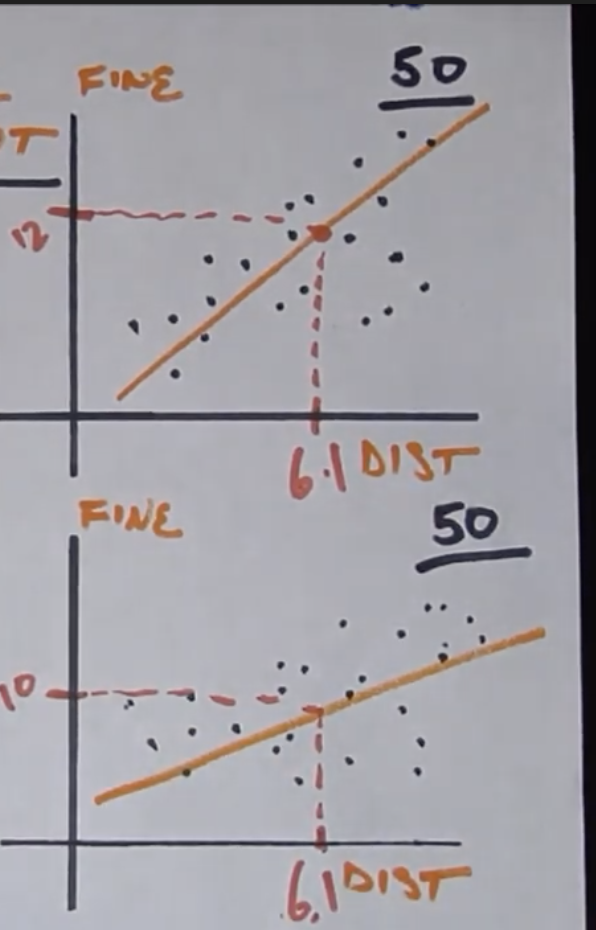
\includegraphics[scale=0.3]{src/ritvikmath-multiple-imputation.png}
		\end{center}
	\item	Cons: complicated.
\end{itemize}
\end{YTB_SUMM_AUTO_NUMB}

\newpage


\section*{Regularisation}

\begin{YTB_vids}[Vidéos YouTube]
\begin{itemize}
	\item	\nameref{SQ-reg-3-elasticnet}
\end{itemize}
\end{YTB_vids}

\begin{YTB_SUMM_AUTO_NUMB}[label = {SQ-reg-3-elasticnet}]{\href{https://www.youtube.com/watch?v=1dKRdX9bfIo&feature=youtu.be}{Regularization Part 3: Elastic Net Regression}}
\begin{itemize}[leftmargin = *]
	\item	Lasso est optimal lorsque le modèle contient beaucoup de variables \textit{inutiles} puisqu'ils les éliminent.
	 		Il permet de créer un modèle plus simple qui sera plus facilement interprétable. 
	\item	En contraste, la régression Ridge est optimale lorsque le modèle contient beaucoup de variables qui sont \textit{majoritairement utiles}. Il permet de réduire l'importance des variables en diminuant leurs coefficients, mais n'ira pas si loin que les éliminer.
	\item	Mais quoi faire lorsqu'il y a encore plus de variables??
	\item	For example, with big data there are millions of variables—far too many to know everything about them.
	\item	So, \hl{when there are many variables you almost certainly need some sort of regularization to estimate parameters}.
	\item	In this scenario, you don't have to choose between Ridge and Lasso instead you just use \textbf{Elastic-Net Regression}.
		\begin{itemize}[leftmargin = *]
		\item	Start with least squares (like Lasso and Ridge).
		\item	Combine the Lasso $\lambda_{1}$ and Ridge $\lambda_{2}$ penalties.
		\end{itemize}
		\begin{align*}
		SS(\text{residuals}) \textbf{\Large{+}} 
		\lambda_{1} |\text{parameter}_{1}| + \dots + |\text{parameter}_{X}| \textbf{\Large{+}}
		\lambda_{2} \text{parameter}_{1}^{2} + \dots + \text{parameter}_{Y}^{2}
		\end{align*}
	\item	The regression penalty coefficients $\lambda_{1}$ and $\lambda_{2}$, use CV.
		\begin{center}
			\begin{tabular}{|	c	|	c	|	c	|}
			\hline
			Lasso parameter		&	Ridge parameter		&	Regression	\\\hline
			$\lambda_{1} = 0$	&	$\lambda_{2} = 0$	&	Ordinary Least Squares 	\\
			$\lambda_{1} > 0$	&	$\lambda_{2} = 0$	&	Lasso 	\\
			$\lambda_{1} = 0$	&	$\lambda_{2} > 0$	&	Ridge 	\\
			$\lambda_{1} > 0$	&	$\lambda_{2} > 0$	&	Elastic Net 	\\\hline
			\end{tabular}
		\end{center}
	\item	Elastic Net is particularly good at dealing with situations where there are correlations between parameters.
		\begin{itemize}
		\item	Lasso tends to pick just one of the correlated terms and eliminate the others.
		\item	Ridge tends to shrink all of the correlated variables parameters together.
		\item	Elastic Net groups and shrinks the correlated variables’ parameters and either leaves them or removes all of them.
		\end{itemize}
\end{itemize}
\end{YTB_SUMM_AUTO_NUMB}

\section*{Trees}

\begin{YTB_vids}[Vidéos YouTube]
\begin{itemize}
	\item	\nameref{SQ-RF-PT1}
	\item	\nameref{SQ-RF-PT2}
	\item	\nameref{SQ-RF-R}
\end{itemize}
\end{YTB_vids}

\begin{YTB_SUMM_AUTO_NUMB}[label = {SQ-RF-PT1}]{\href{https://www.youtube.com/watch?v=J4Wdy0Wc_xQ&feature=youtu.be}{StatQuest: Random Forests Part 1 - Building, Using and Evaluating}}
\begin{itemize}[leftmargin = *]
	\item	The only caveat of CARTs are that they are very inaccurate for new data.
	\item	Thus, random forests permit us to combine the simplicity of decision trees with flexibility for much better accuracy.
	\item	To create a random forest:
		\begin{itemize}[leftmargin = *]
		\item	Create a bootstrapped dataset.
		\item	Create a decision tree with the bootstrapped dataset only considering a random subset of the variables at each step.
		\item	Repeat with a new bootstrapped dataset (usually hundreds of times).
		\item	To get a prediction, we run our observation through the decision trees and the result with the most votes is the prediction:
		\begin{center}
			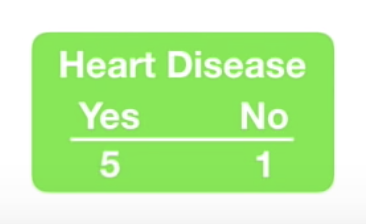
\includegraphics[scale=0.4]{src/SQ-RF-VOTE.png}
		\end{center}
		\end{itemize}
	\item	This provides a much wider variety of decision trees which is why random forests are much more flexible.
	\item[]	\textbf{Note}: \textbf{B}ootstrapping the data and using the \textbf{agg}regate to make a decision is called \textbf{bagg}ing.
	\begin{itemize}[leftmargin = *]
		\item	Typically about $1/3$ of the original data does not end up in the bootstrapped dataset---this is the \textbf{Out-Of-Bag} dataset.
		\item	A better terminology, however, would be the \textbf{Out-Of-Boot} dataset as it's the data which wasn't in the bootstrapped dataset.
		\item	It becomes our testing dataset with which we calculate the \textbf{Out-Of-Bag Error}.
	\end{itemize}
	\item	We do this with a different number of variables being used per step to find the optimal number of variables to use.
	\item	Typically, we start with the square of the number of variables and try a few settings above and below that value.
\end{itemize}
\end{YTB_SUMM_AUTO_NUMB}

\begin{YTB_SUMM_AUTO_NUMB}[label = {SQ-RF-PT2}]{\href{https://www.youtube.com/watch?v=sQ870aTKqiM&feature=youtu.be}{StatQuest: Random Forests Part 2: Missing data and clustering}}
\begin{itemize}[leftmargin = *]
	\item	Random forests consider 2 types of missing data:
		\begin{enumerate}[leftmargin = *]
		\item	Missing data in the original data set used to create the RF.
			\begin{itemize}[leftmargin = *]
			\item	The idea is to make an initial guess that could be bad, then gradually refine the guess until it is (hopefully) a good guess.
			\item	The initial bad guess is to input the most common value for a categorical variable, and the median for a numeric one.
			\item	To refine the guess, we find observations which are \textit{similar} to the one with missing data.
			\item	In the case of a RF, samples which end up in the same terminal node are \textit{similar}.
			\item	We can keep track of similar samples with a proximity matrix.
			\item	After each iteration of the RF, we add one to the samples which end up together and then divide the total by the number of trees.
			\begin{center}
				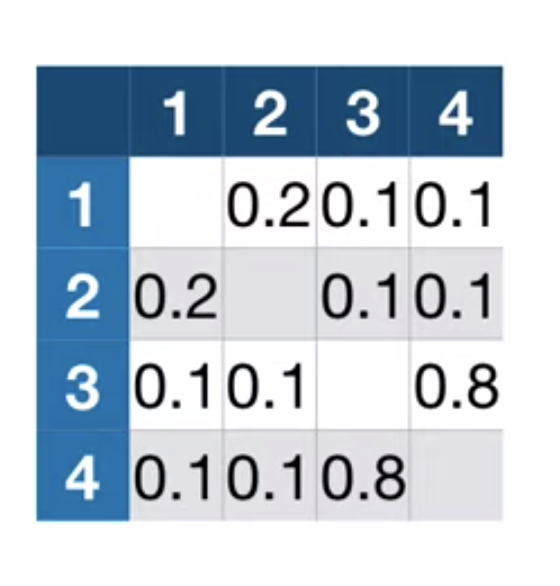
\includegraphics[scale=0.4]{src/SQ-proximity-matrix.png}
			\end{center}
			\item	Therefore we can make better guesses about the missing data using proximity values to weigh the frequency of different values.
			\item	weight for the sample 4 yes = $\frac{\text{proximity where yes}}{all proximities for sample 4}$.
			\item	Can find the distance matrix which is $1 - proximity$ and them do heat maps or MDS / PCoA.
			\end{itemize}
		\item	Missing data in a new sample we want to categorize.
			\begin{itemize}[leftmargin = *]
			\item	Create two copies of the observation---Yes and No.
			\item	Then, use the same method to input the missing data.
			\item	Then, take the option which classifies the best as either Yes or No respectively.
			\end{itemize}
		\end{enumerate}
\end{itemize}
\end{YTB_SUMM_AUTO_NUMB}

\begin{YTB_SUMM_AUTO_NUMB}[label = {SQ-RF-R}]{\href{https://www.youtube.com/watch?v=6EXPYzbfLCE&feature=youtu.be}{StatQuest: Random Forests in R}}
\begin{itemize}[leftmargin = *]
	\item	package \texttt{randomForest}.
	\item	Default number of splits is the square root of the number of variables.
	\item	Plot the error rates to determine the number of trees for optimal classification.
\end{itemize}
\end{YTB_SUMM_AUTO_NUMB}

\section*{Boosting}

\begin{YTB_vids}[Vidéos YouTube]
\begin{itemize}
	\item	\nameref{SQ-Boo-Ada}
	\item	\nameref{SQ-Boo-Reg-Idea}
	\item	\nameref{SQ-desc-grad}
	\item	\nameref{SQ-desc-grad-sto}
	\item	\nameref{SQ-Boo-Reg-Det}
	\item	\nameref{SQ-Boo-Class-Idea}
	\item	\nameref{SQ-Boo-Class-Det}
\end{itemize}
\end{YTB_vids}


\begin{YTB_SUMM_AUTO_NUMB}[label = {SQ-Boo-Ada}]{\href{https://www.youtube.com/watch?v=LsK-xG1cLYA&feature=youtu.be}{AdaBoost, Clearly Explained}}
\textbf{\underline{Differences between Random Forests and Adaboost}}

\textbf{Random Forest}
\begin{itemize}[leftmargin = *]
	\item	Each time you make a tree, you make a full sized tree.
		\begin{itemize}[leftmargin = *]
		\item	Some trees may be bigger than others, but there's \textbf{no predetermined maximum depth}.
		\end{itemize}
	\item	Each tree has an equal vote on the final classification.
	\item	Each tree is made independently of the others.
\end{itemize}

\textbf{Adaboost Random Forest}
\begin{itemize}[leftmargin = *]
	\item	Trees are usually \textit{just one node} and \textit{two leaves}---a \textbf{stump}.
		\begin{itemize}[leftmargin = *]
		\item	So Adaboost is really a random "\textit{Forest of Stumps}".
		\item	Stumps are not great at making classifications as they only have one variable to make a decision---they are "\textit{weak learners}".
		\end{itemize}
	\item	Some stumps get more say than others in the final classification.
	\item	Trees are mare sequentially thus order has an impact.
		\begin{itemize}[leftmargin = *]
		\item	The first stump's errors influences how the second stump is made.
		\end{itemize}
\end{itemize}

\tcbline

\textbf{Procedure}:
\begin{enumerate}[leftmargin = *]
\item	We give each observation, or \textit{sample}, a \textbf{"sample" weight} to indicate how important it is that it be correctly classified.	
\begin{itemize}
	\item	Initially, all samples get the same weight $\frac{1}{\text{total number of samples}}$.
	\item	However, after making the first stump, these weights will change in order to guide how the next stump is created.
\end{itemize}

\item	To make the first stump, we find the variable which does the best job classifying the sample.
\begin{itemize}
	\item	Given all the weights are the same right now, we can ignore them.
	\item	We could use the Gini index to compare the variables.
\end{itemize}

\item	We determine how much say the first stump will have in the final classification.
\begin{itemize}
	\item	The \textbf{total error} for a stump is the sum of the "sample" weights associated with the incorrectly classified samples.
		\begin{itemize}[leftmargin = *]
		\item	For example, incorrectly classifying 2 samples with sample weights of 1/8 leads to a total error of 2/8.
		\item	Given the sample weights add up to 1, the total error will always be between 0 (a perfect stump) and 1 (a terrible stump).
		\end{itemize}
	\item	The \textbf{amount of say} = $\frac{1}{2} \log \left( \frac{1 - \text{Total Error}}{\text{Total Error}} \right)$.
	\item[]	Its graph looks like this:
	\begin{center}
		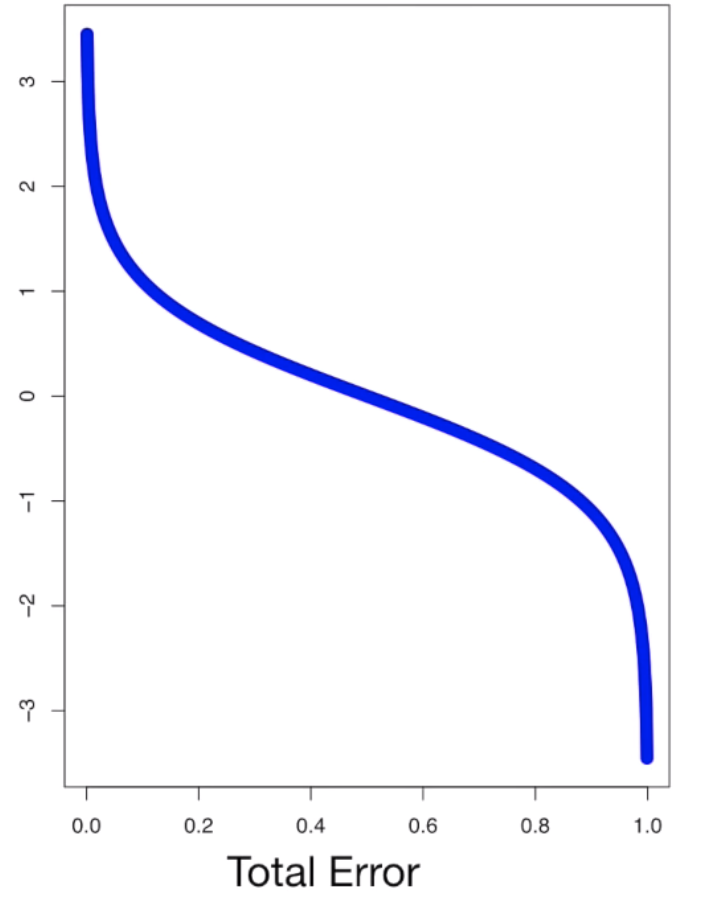
\includegraphics[scale=0.4]{src/SQ-ADA-AMT-SAY.png}
	\end{center}
		\begin{itemize}[leftmargin = *]
		\item	When a stump is efficient and has a relatively small total error, its amount of say will be relatively large.
		\item	If a stump is really bad, the negative value will turn a "Yes" into a "No".
		\end{itemize}
	\item	In brief, the sample weights from \textit{\textbf{incorrectly}} classified samples determine the \textit{amount of say} each stump gets.
\end{itemize}

\item	Modify the weights so that the next stump will account for the previous stump's errors.
\begin{itemize}[leftmargin = *]
	\item	Originally all the sample weights were identical.
	\item[]	Therefore, there was no emphasis on the \textit{importance of correctly classifying} any one particular sample.
	\item[]	However, we really want the samples (observations) which were incorrectly classified before to be correctly classified in the next stump. 
	\item[]	So, we give the incorrectly classified samples more weight and reduce the weight of the samples that were correctly classified.
	\item	When we want to \textit{\textbf{increase}} the weights, the \textbf{new sample weight} = $\text{sample weight} \times \textrm{e}^{\text{amount of say}}$.
	\item[]	Its graph looks like this:
	\begin{center}
		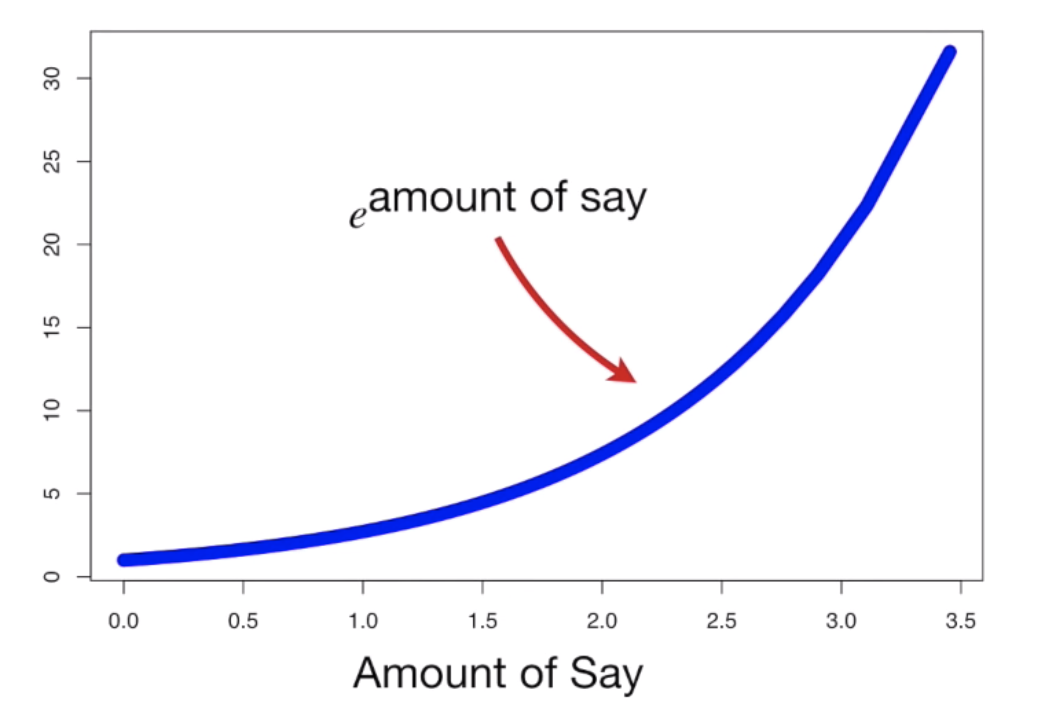
\includegraphics[scale=0.4]{src/SQ-ADA-NEW-SWE.png}
	\end{center}
		\begin{itemize}[leftmargin = *]
		\item	When a stump is efficient and has a relatively high amount of say, then the new sample weight will be much larger than the previous.
		\item	If a stump is really bad, then the new sample weight will not change very much.
		\end{itemize}
	\item	When we want to \textit{\textbf{\textcolor{red}{decrease}}} the weights, the \textbf{new sample weight} = $\text{sample weight} \times \textrm{e}^{\textcolor{red}{-}\text{amount of say}}$.
	\item	We then normalize them so they're between 0 and 1 with $\frac{\text{sample weight}}{\text{sum of the new sample weights}}$.
	\item	Theoretically, these weights could be used to calculate the weighted Gini index.
	\item	Instead, we make a new sample of the same size picking observations according to their weight using the inversion method.
		\begin{itemize}[leftmargin = *]
		\item	Thus, some observations could (should) be repeated in the new sample set.
		\item	Then, we give equal weights to this new sample.
		\item	Because some observations will be repeated, they will have a higher weight as the will be treated like a "block" with a large penalty for misclassification.
		\end{itemize}
\end{itemize}

\item	Predict
\begin{itemize}[leftmargin = *]
	\item	We sum the amount of say from each root tree and the class having the highest weight is the predicted value.
\end{itemize}
\end{enumerate}

\tcbline

\textbf{\underline{Three main ideas}}:
\begin{enumerate}[leftmargin = *]
	\item	\textbf{Adaboost} combines a lot of \textit{weak learners} to make classifications.
		\begin{itemize}[leftmargin = *]
		\item	The weak learners are almost always \textbf{stumps}.
		\end{itemize}
	\item	Some \textbf{stumps} get more say in the classification than others.
	\item	Each \textbf{stump} is made by taking the previous \textbf{stump's} mistakes into account.
		\begin{itemize}[leftmargin = *]
		\item	If we have a \textit{weighted Gini function}, then we use it with the sample weights.
		\item	Otherwise, we use the sample weights to make a new dataset reflect them (generate  a number between 0 and 1, choose observation according to the cumulative proportion).
		\end{itemize}
\end{enumerate}
\end{YTB_SUMM_AUTO_NUMB}

\begin{YTB_SUMM_AUTO_NUMB}[label = {SQ-Boo-Reg-Idea}]{\href{https://www.youtube.com/watch?v=3CC4N4z3GJc&feature=youtu.be}{Gradient Boost Part 1: Regression Main Ideas}}
\textbf{Comparison / general details} 
Gradient boost
\begin{enumerate}[leftmargin = *]
	\item	Make a single leaf, instead of a tree or a stump.
	\begin{itemize}[leftmargin = *]
	\item	The leaf represents an initial guess for the weights of all the samples.
	\item	When trying to predict a continuous value, the first guess is the average value.
	\end{itemize}
	\item	Build a tree
	\begin{itemize}[leftmargin = *]
	\item	Like Adaboost, usually based on the previous tree's errors.      
	\item	Unlike Adaboost, the tree is usually larger than a stump.        
	\item	Gradient boost does however restrict the size of the tree.       
		\begin{itemize}[leftmargin = *]
		\item	Often the maximum number of leaves is between 8 and 32.
		\end{itemize}
	\item	It scales all trees by the same amount.
	\end{itemize}
\end{enumerate}

\tcbline

\textbf{Procedure}

\begin{enumerate}[leftmargin = *]
	\item	Calculate the average weight = 71.2kg.
	\begin{itemize}[leftmargin = *]
	\item	First "attempt" at predicting everyone's weight; i.e., if we stopped right now, we'd predict that everyone weighs 71.2 kg.
	\end{itemize}

	\item	Build a tree based on the errors the previous tree made.
	\begin{itemize}[leftmargin = *]
	\item	The error, or \textbf{pseudo-residual}, is the difference between the observed $x$ and predicted $\bar{x}$ weights $x - \bar{x}$.
		\begin{itemize}[leftmargin = *]
		\item	"Residual" is based on linear regression's residuals between the curve and real data points.
		\end{itemize}
	\end{itemize}

	\item	We use the variables to \textbf{predict the residuals}.
	\begin{itemize}[leftmargin = *]
	\item	The tree will predict the average of the residuals from the observations in the leaf.
	\begin{itemize}[leftmargin = *]
	\item	So, with an initial prediction of 71.2 ($\bar{x}$), the predicted weight is (for example) $71.2 + 16.8 = 88$.
	\item	In this case, the prediction is bad because it is overfit---low bias and high variance.
	\end{itemize}
	\item	We address this with a learning rate $\lambda$ which scales the value.
	\begin{itemize}[leftmargin = *]
	\item	For example, the predicted weight would be $71.2 + 0.10 \times  16.8 = 72.9$.
	\item	The prediction is a \textbf{little worse} than before but a \textbf{little better} than the initial guess of 71.2.
	\end{itemize}
	\item	So, we take \textbf{many little steps} in the right direction for better predictions and see this by having slightly smaller residuals.
	\end{itemize}

	\item	We repeat with the new tree.
	\begin{itemize}[leftmargin = *]
	\item	For example, we'd predict $71.2 + 0.1 \times 16.8 + 0.1 \times 15.1 = 74.4$.
	\end{itemize}
\end{enumerate}
\end{YTB_SUMM_AUTO_NUMB}

\begin{YTB_SUMM_AUTO_NUMB}[label = {SQ-desc-grad}]{\href{https://www.youtube.com/watch?v=sDv4f4s2SB8}{Gradient Descent, Step-by-Step}}
\begin{itemize}[leftmargin = *]
	\item	Examples of times we optimize:
		\begin{itemize}[leftmargin = *]
		\item	Linear regression: we optimize the intercept and slope when fitting a line.
		\item	Logistics regression: we optimize a squiggle.
		\end{itemize}
	\item	\textbf{Gradient descent} can optimize \textit{all} of this \underline{and more}.
	\item	To optimize the intercept when fitting a line with gradient descent:
		\begin{enumerate}[leftmargin = *]
		\item	Pick a random value for the intercept.
			\begin{itemize}[leftmargin = *]
			\item	This initial guess gives gradient descent something to improve upon.	
			\end{itemize}
		\item	Evaluate how well the line fits the data with the SSR.
			\begin{itemize}[leftmargin = *]
			\item	In machine learning, we refer to the SSR as a type of \textbf{Loss Function}.
			\end{itemize}
		\item	Repeat this with several possible values for the intercept and plot the SSR in function of the intercept:
			\begin{center}
			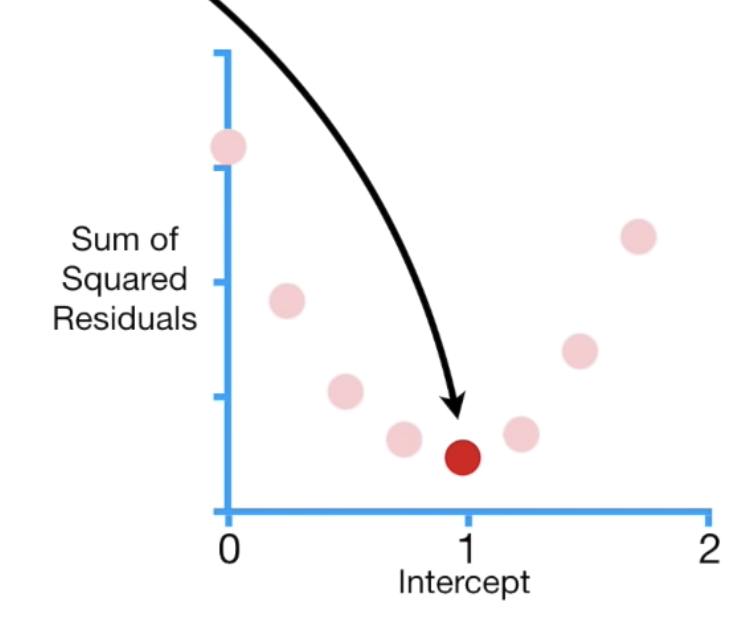
\includegraphics[scale=0.4]{src/SQ-GD-SSR.png}
			\end{center}
		\end{enumerate}
		\begin{itemize}
		\item	The long way to then find the optimal intercept and find the best value would be to test the values between the lowest points to see if another number is better.
		\item	Gradient descent does a few calculations far from the optimal solution and increases the number as it gets closer to the optimal one:
		\begin{center}
			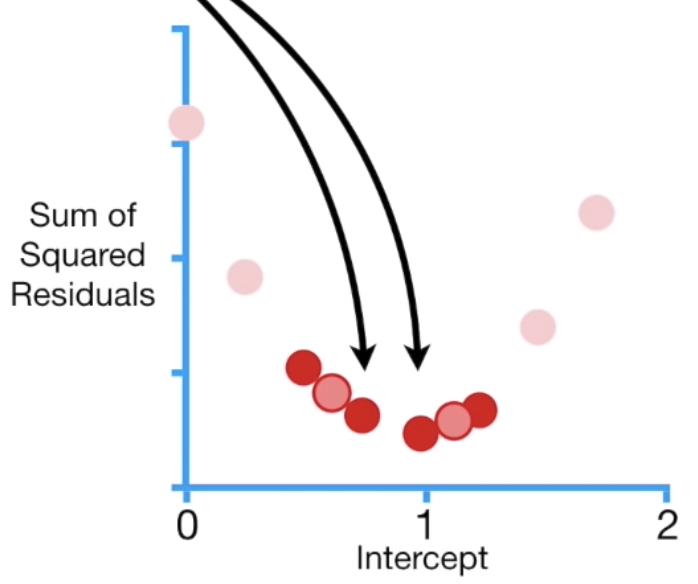
\includegraphics[scale=0.4]{src/SQ-GD-SSR-2.png}
		\end{center}
			i.e., it takes big steps when far away and baby steps when it is close.
		\end{itemize}
	\item	To optimize the intercept, we develop SSR as a function of the intercept:
		\begin{center}
		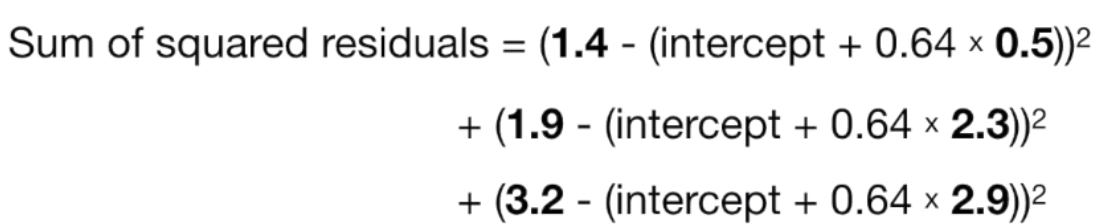
\includegraphics[scale=0.4]{src/SQ-GD-SSR-3.png}
		\end{center}
	\item	Then, we take it's derivative so that \textbf{Gradient Descent} can use it to find the point where the slope is 0.
	\item	In linear regression, find where the slope is 0 but gradient descent tries values sequentially:
		\begin{center}
		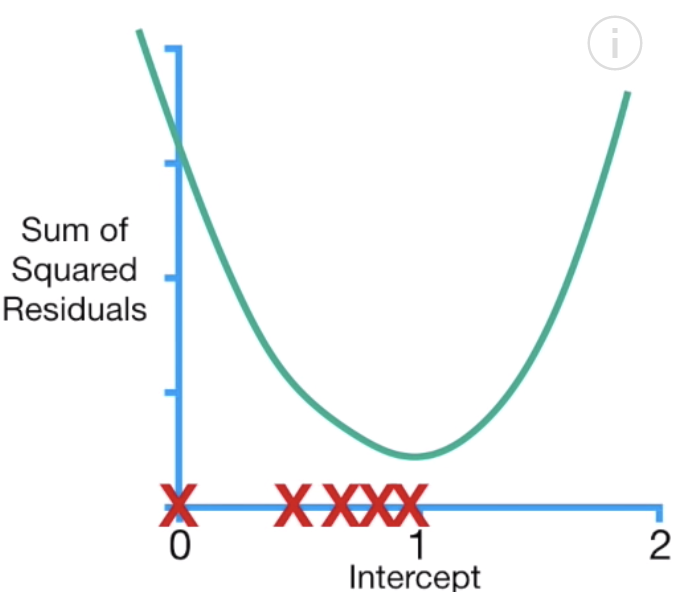
\includegraphics[scale=0.4]{src/SQ-GD-SSR-4.png}
		\end{center}
	\item	Step size = $\text{slope} \times \text{learning rate}$ and new intercept = old intercept  - step size.
	\item	It stops taking steps when the step size is very close to 0, in practice it is often 0.001 or less, or when it reaches a maximum number of steps.
	\item	To optimize find the slope \textbf{AND} intercept, we take the derivative with respect to both.
	\item	When you have multiple derivatives of the same function, they're referred to as the "\textbf{gradient}" of a function.
	\item	We use the \textbf{gradient} to \textbf{descend} to the lowest point of the \textbf{loss function}.
	\item	Gradient descent is very sensitive to the learning rate---in practice, we start large and try lower and lower values until we converge.
\end{itemize}
\tcbline
\textbf{In brief}
\begin{enumerate}
	\item	Take the derivative of the \textbf{Loss Function} for each parameter in it.
	\item	Pick random values for the parameters.
	\item	Plug the parameter values into the derivatives (the gradient).
	\item	Calculate the step sizes: \textbf{step size} = \textbf{slope} $\times$ \textbf{learning rate}.
	\item	Calculate the new parameters: \textbf{new parameter} = \textbf{old parameter} -  \textbf{step size}
	\item	Repeat from step 3 until the step size is very small, or you reach the maximum number of steps.
\end{enumerate}

With many data points, it can be very long to calculate the SSR at each step. \textbf{Stochastic Gradient Descent} uses a random subset of the data at every step instead of the full dataset.
\end{YTB_SUMM_AUTO_NUMB}

\begin{YTB_SUMM_AUTO_NUMB}[label = {SQ-desc-grad-sto}]{\href{https://www.youtube.com/watch?v=vMh0zPT0tLI}{Stochastic Gradient Descent, Clearly Explained!!!}}
\begin{itemize}[leftmargin = *]
	\item	The main advantage of stochastic gradient descent is to apply gradient descent to a large amount of data. 
	\item	For example, with only 10'000 data points, we'd already have to calculate 20'000 residuals \textit{at every step}.
	\item	Stochastic Gradient Descent is also very sensitive to the learning rate and we also start large and get progressively smaller. The way the rate changes is called the \textbf{schedule}.
	\item	It is especially useful when there are redundancies in the data.
	\item	The \textbf{strict} definition is to use 1 observation per step.\\
			However, it is more common to use a small subset, or \textbf{mini-batch}, of data for each step.
	\item	It can lead to more stable estimates of the parameters in fewer steps.
	\item	An advantage of Stochastic Gradient Descent is we can use it to adjust our guess instead of restarting the whole process.
\end{itemize}
\end{YTB_SUMM_AUTO_NUMB}

\begin{YTB_SUMM_AUTO_NUMB}[label = {SQ-Boo-Reg-Det}]{\href{https://www.youtube.com/watch?v=2xudPOBz-vs&feature=youtu.be}{Gradient Boost Part 2: Regression Details}}
The formula looks complicated because it's designed to be applicable in many situations.
\begin{itemize}[leftmargin = *]
	\item	
\end{itemize}
\end{YTB_SUMM_AUTO_NUMB}

\begin{YTB_SUMM_AUTO_NUMB}[label = {SQ-Boo-Class-Idea}]{\href{https://www.youtube.com/watch?v=jxuNLH5dXCs&feature=youtu.be}{Gradient Boost Part 3: Classification}}

\begin{itemize}[leftmargin = *]
	\item	
\end{itemize}
\end{YTB_SUMM_AUTO_NUMB}

\begin{YTB_SUMM_AUTO_NUMB}[label = {SQ-Boo-Class-Det}]{\href{https://www.youtube.com/watch?v=StWY5QWMXCw&feature=youtu.be}{Gradient Boost Part 4: Classification Details}}

\begin{itemize}[leftmargin = *]
	\item	
\end{itemize}
\end{YTB_SUMM_AUTO_NUMB}

\end{document}
